\documentclass[10pt,a4paper]{article}
\usepackage[T1]{fontenc}
\usepackage[utf8x]{inputenc}
\usepackage{ucs}
\usepackage[english,catalan,spanish]{babel}
\usepackage{times}
\usepackage{graphicx}
\usepackage{subfigure}
\usepackage{listings}
\usepackage{moreverb}
\usepackage{hyperref} % option [dvipdfm] disables clickable refs
\hypersetup{pdftex, colorlinks=true, linkcolor=blue, filecolor=blue,pagecolor=blue, urlcolor=blue}

%% The default sizes of LaTeX is too small. It is better to put more
%% \setlength{\textwidth}{6.78in}
%% \setlength{\textheight}{8.9in}
%% \setlength{\hoffset}{-0.25in} % 0,75in margin
%% \setlength{\voffset}{-0.50in} % 0,50in margin
%% \setlength{\oddsidemargin}{0in}
%% \setlength{\evensidemargin}{\oddsidemargin}
%% \setlength{\headheight}{0.0in}
%% \setlength{\footskip}{0.60in}
%% \setlength{\headsep}{0.21in}

\newcommand{\partikle}[0]{\texttt{PaRTiKle}}
\newcommand{\xtratum}[0]{\texttt{XtratuM}}
\newcommand{\hrefx}[1]{\href{#1}{#1}} % explicit \href
\newenvironment{itemize*}
        {\begin{itemize}%
                \setlength{\parskip}{2pt}%
                \setlength{\itemsep}{0pt}}
        {\end{itemize}}
\newenvironment{enumerate*}
        {\begin{enumerate}%
                \setlength{\parskip}{2pt}%
                \setlength{\itemsep}{0pt}}
        {\end{enumerate}}

\title{Manual del usuario:\\
	\partikle{} sobre sistemas LPC2000}

\author {S. Peiró\\ \small{Rev: Miguel Masmano}\\%
	Grupo de Informática Industrial y Sistemas de Tiempo Real\\
	Universidad Politécnica de Valencia, Spain\\
\{speiro,mmasmano\}@ai2.upv.es
}

\begin{document}

\maketitle

\begin{abstract}
	En este texto se describe la puesta a punto desde cero del entorno de programación para desarrollar aplicaciones que se ejecuten sobre los sistemas LPC2000 con el SOTR \partikle{} \cite{partikleos}.
	Dentro del entorno de programación se contempla tanto la parte hardware como la parte software:
	
	 \begin{description}
	 \item[Hardware]
	 El sistema LPC2000 y los dispositivos necesarios para tener acceso desde una terminal serie (\emph{host}) hasta el LPC2000 (\emph{target}). 

	%Esto incluye tanto los drivers para la parte del PC (\emph{host}) que se va a utilizar programar así como la parte requerida por el LPC2000.

	 \item[Software]
	 El sistema operativo de tiempo real para sistemas empotrados \partikle{} \cite{partikleos}, las herramientas de compilación (\emph{toolchain}) y el cargador por puerto serie utilizado para cargar código en el LPC2000.
	 \end{description}

\end{abstract}

\begin{center}
\textbf{Keywords:}
	\newblock {PaRTiKle, Real Time Operating Systems, LPC200, ARM7, System Programming}
\end{center}

\tableofcontents

\newpage

\section{Sistemas LPC2000}

	Este apartado presenta una visión general de los sistemas utilizados, proporcionando referencias a documentos más específicos que quedan fuera del alcance de este manual.  El manual se centra en particular en el modelo LPC2136 que utiliza los procesadores de la arquitectura ARM (\emph{Advanced RISC Machines}) de 32 bits, en particular la familia ARM7TDMI-S, donde la S final hace referencia a que el procesador esta modelado en VHDL.
	
	\subsection{Características LPC2000}
	
	A continuación se muestran las características generales del modelo LPC2136:
		
	\begin{table}[ht]
	\centering
	\begin{tabular}{|l|l|} \hline
	Modelo		&	LPC2136  \\ \hline
	Procesador	&	ARM7TDMI-S 60 Mhz \\ \hline
	Memoria  RAM	&	32 Kbytes (expandible módulo externo)\\ \hline
	Memoria  ROM	&	256 Kbytes EEPROM (electrically-erasable programmable ROM)\\ \hline
	Puertos serie	&	UART0: serial (38400 bauds) + UART1: modem \\ \hline
	Relojes		&	RTC 32.768 KHz \\ \hline
	Timers		&	t0, t1:  ~ 15Mhz (CCLK= 60 Mhz / PDIV = 4) \\ \hline
	Otros		&	gpio, spi, pwm, i2c, can, ... \\ \hline
	\end{tabular}
	
	\caption{Resumen de especificaciones LPC2136}
	\label{fig:resumen}
	\end{table}
	
	En la figura \ref{fig:lpc-ubirov2} se puede ver la placa utilizada en el robot
	de tipo humanoide: \emph{$\mu$biro v2} (20 º de libertad para el movimiento del robot)
	este robot incorpora el sistema LPC2136 sobre el que se ha portado el sistema operativo \partikle{}.
	
	La placa ha sido diseñada en el Grupo de Informática Industrial en el Instituto de Automática e Informática industrial (\hrefx{http://www.ai2.upv.es}).
	Se puede encontrar más detalles, así como videos del robot  \emph{$\mu$biro v2} en funcionamiento
	en la siguiente dirección \hrefx{http://www.gii.upv.es/personal/mialgil/ubiro2.htm}
	
	\begin{figure}[htbp]
	\begin{center}
	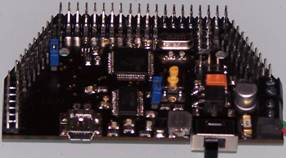
\includegraphics[width = 0.8\columnwidth]{img/lpc-ubirov2}
	\end{center}
	
	\caption{Placa utilizada por \emph{$\mu$biro v2}}
	\label{fig:lpc-ubirov2}
	\end{figure}
	
	Para una descripción más detallada de las características del LPC2136 se puede ver su manual del usuario~\cite{lpc213x-um}, así como el manual del procesador ARM7TDMI~\cite{arm7tdmi-s}. Por otra parte para cuestiones generales sobre la arquitectura ARM ver el \emph{Architecture Reference Manual} \cite{armarm}.
	
	A continuación a modo de introducción se presentan una serie de secciones que tratan los aspectos básicos de la programación de los sistemas LPC2000. En estas secciones se da respuesta a dos preguntas básicas: el procedimiento para arrancar al procesador y el procedimiento de carga de código para su posterior ejecución.
	
	\subsubsection{Inicialización}
	
	Al poner en funcionamiento el procesador, este comienza a ejecutar código en el vector de interrupción de reset \texttt{vector[reset]}. Abajo se pueden ver las distintas causas de interrupción que puede recibir el procesador, junto con los vectores de interrupción a cargar en cada caso y sus direcciones de memoria:

	\begin{figure}[htbp]
	\centering

	\begin{boxedverbatim}
	# entradas      # direcciones  # propósito
	vector[reset]   0x00000000     Reset
	vector[undf]    0x00000004     Undefined Instruction
	vector[swi]     0x00000008     Software interrupt
	vector[pabt]    0x00000010     Program abort
	vector[dabt]    0x00000014     Data abort
	vector[cksum]   0x00000018     Reserved: checksum
	vector[irq]     0x0000001c     Interrupt ReQuest
	vector[fiq]     0x00000020     Fast Interrupt reQuest
	\end{boxedverbatim}
	\caption{Vectores de interrupción ARM}\label{fig:vector}
	\end{figure}
	
	Tras un reset el procesador asigna al contador de pograma (PC) la dirección del vector de interrupción de reset \texttt{vector[reset]}. Como resultado de esto se comienza a ejecutar la instrucción que se encuentre en \texttt{PC = 0x00000000}. El \texttt{vector[reset]} es el encargado de inicializar el LPC2000 en el siguiente orden:
	
	\begin{itemize*}
	\item Código de arranque, programación PLL, \ldots
	\item Inicialización de los modos de interrupción, reservar pilas de programa (stacks), \ldots
	\item Interrupciones, configurar las interrupciones para su uso.
	\item Dispositivos: en particular el puerto serie para poder depurar el código que estamos ejecutando.
	\end{itemize*}
	
	\paragraph{Inicialización de los modos de interrupción}
	
	Las restantes entradas del vector de interrupción también deben de inicializarse, ya que se encargan de la gestión de interrupciones (IRQ, FIQ) y excepciones: (Undefined, Data Abort, Program Abort, etc.) que es interesante tratar para presentar un volcado del estado del procesador: registros y pila, para tener información suficiente para comprender las causas de la excepción.

	\paragraph{Reserva de pilas de programa}
	
	El estándar del procedimiento de llamadas a funciones de C para la arquitectura ARM ATPCS \cite{ATCPS}, requiere de un puntero a una pila de memoria para proporcionar los bloques de activación (almacenamiento de variables locales, temporales, \ldots) de las funciones en C.
	
	Para ello es necesario durante la inicialización del procesador proporcionar una zona de memoria suficientemente grande para la pila del modo funcionamiento del procesador SVC.
	
	En caso de no ser así, y si el tamaño reservado para dicha pila fuera inferior al utilizado, el sistema comenzaría a utilizar zonas de memoria no reservada, con lo que dejaría de funcionar correctamente. En dicho caso se pueden editar los fuentes para ampliar el tamaño de la pila SVC.
	
	\subsubsection{Interrupciones}
	
	Para gestionar los dispositivos de los LPC2000 se utiliza el modelo de peticiones de interrupción, de forma que el procesador se encuentra en su hilo de ejecución, y cuando alguno de los dispositivos requiere la atención del procesador, realiza una petición de interrupción que el procesador puede atender. Para ello el procesador ARM unicamente proporciona los modos de funcionamiento IRQ y FIQ, el resto es tarea del sistema específico.

	Así pues los sistemas ARM incorporan un controlador de interrupciones, que se encarga de notificar al procesador de las interrupciones y proporcionar una interfaz para su acceso/control desde el procesador. En el caso del LPC2000, este controlador se implementa mediante el VIC (\emph{Virtual Interrupt Controller}).
	
	
	\begin{figure}[htbp]
	\begin{center}
	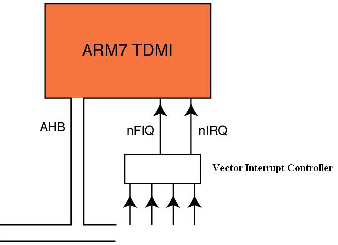
\includegraphics[width = 0.3\columnwidth]{img/lpcvic}
	\end{center}
	
	\caption{Controlador VIC LPC2000}
	\label{fig:lpcvic}
	\end{figure}
	
	El VIC presenta un conjunto de registros (mapeados en la memoria del ARM7) para acceder/controlar las interrupciones de los distintos dispositivos disponibles en el LPC2000, por medio de escrituras/lecturas en memoria.
	Cuando se recibe una interrupción el procesador carga en el PC la entrada correspondiente del vector de interrupción (\texttt{vector[irq]}).  Esta a su vez será una instrucción de salto o modificación del PC, en el caso de las IRQ, FIQ se trata de un salto a un manejador de interrupciones global encargado de determinar la interrupción del dispositivo específico que se ha producido y ejecutar su manejador asociado.
		
	\subsubsection{Uart serie}
		
	Los LPC2000 incorporan dos uarts en el chip, las dos son idénticas en cuanto a su modo de uso, con la excepción de que la UART1 proporciona un soporte adicional para el uso de un MODEM. Ambos periféricos cumplen la especificación ``estándar industrial $550$'' \cite{UART}. Ambas contiene un generador de baud rate y fifos de $16$ bytes para agilizar la recepción/transmisión de carácteres.
	
	\begin{figure}[htbp]
	\begin{center}
	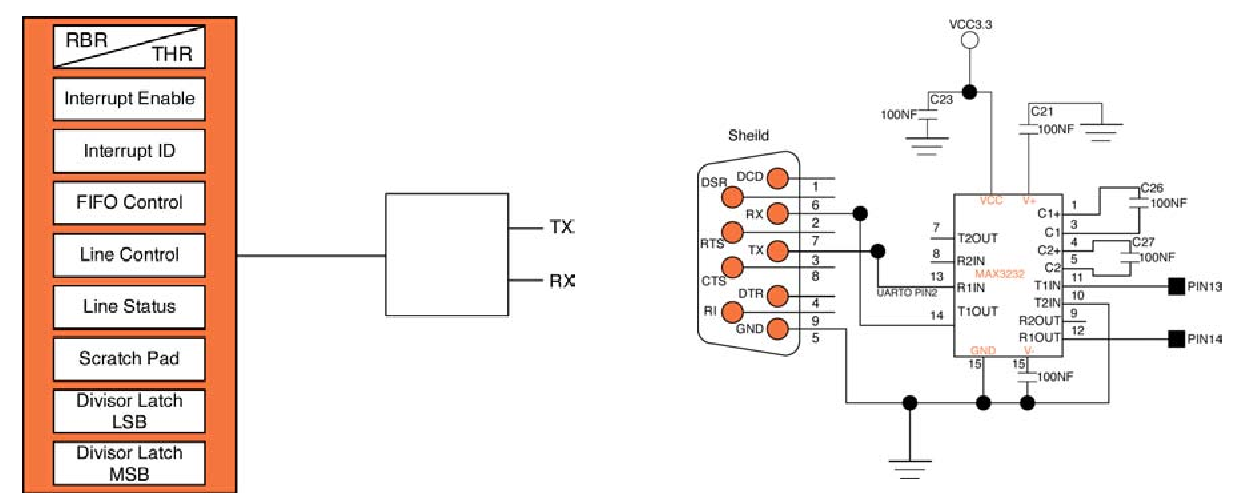
\includegraphics[width = 0.5\columnwidth]{img/lpcuart}
	\end{center}
	
	\caption{UARTs serie presentes en el LPC2000}
	\label{fig:lpcuart}
	\end{figure}
		
	\subsubsection{Gestión de tiempo}

	Los LPC2000 incluyen para la gestión del tiempo un reloj (RTC) y dos temporizadores (T0 y T1).

	El RTC (\emph{Real Time Clock}) que funciona a una frecuencia de $32$Khz como reloj del sistema. La resolución de este reloj es de $(1 / 32 Khz) = 3.05 \cdot 10^{-5}$ sec.

	Los temporizadores T0 y T1 pueden ser utilizados tanto como temporizadores como contadores. Estos funcionan a la frecuencia del bus de periféricos PCLK (\emph{Peripheral bus Clock}) que se calcula de la siguiente forma:

	\begin{eqnarray*}
	        & & CCLK = 60 \cdot 10^6 = 60 Mhz \\
	        & & PDIV	= 4 \\
	        & & PCLK = CCLK / PDIV = 15 \cdot 10^6 = 15 Mhz \\
	\end{eqnarray*}
	Que proporciona una resolución de $6.66 \cdot 10^{-8}$ sec.
	
	\subsubsection{JTAG/ETM}

	Un aspecto importante de estos dispositivos es que proporcionan interfaces para facilitar las tareas de depuración/testing, las cuales suelen ser necesarias en las etapas iniciales de programación. En el caso de LPC2000 se puede utilizar un debugger como GDB/Insight/OpenOCD para acceder al dispositivo a traves de la interfaz JTAG (\emph{Joint Test Action Group}): \hrefx{http://www.google.es/search?q=LPC2000+with+JTAG+gdb+insight}

	En caso de no disponer de debugger, se utiliza la depuración por medio de \texttt{printf()} por el puerto serie.

	\newpage
	
	\section{Entorno de programación}
	
	En este apartado se comenta la puesta a punto desde cero de un entorno de programación para desarrollar aplicaciones sobre el sistema operativo embarcado PaRTiKle.
	
	En este apartado se contemplan las tareas de:
	\begin{itemize*}
	\item Configuración del compilador,
	\item Configuración del cargador flash,
	\item Configuración de \partikle{},
	\item Y por último la compilación y ejecución de aplicaciones sobre \partikle{}.
	\end{itemize*}
	
	\subsection{Configuración compilador}
	
	Para programar el LPC2000 es necesario tener un conjunto de herramientas (compilador, linker, ensamblador, ...) que permitan generar código para el juego de instrucciones Arm/Thumb del procesador. Para ello se utiliza el compilador cruzado (host: x86, target: arm) del proyecto GCC, que permite generar código para el procesador arm7tdmi-s.
	
	El compilador utilizado para compilar \partikle{} para el LPC2000 se ha obtenido de \hrefx{http://www.mikrocontroller.net}~\cite{mikro}. Los pasos para preparar el entorno de compilación utilizado por \partikle{} asumen que el directorio raiz del compilador se encuentre en \texttt{/usr/local/arm/lpc}. Podemos descargar los fuentes del compilador con los siguientes comandos:
	
	\begin{verbatim}
	$ # fuente: http://www.mikrocontroller.net
	$ wget http://www.mikrocontroller.net/download/\
	       arm-toolchain-linux-2.tar.bz2
	$ tar xjvf arm-toolchain-linux-2.tar.bz2 -C /usr/local/
	$ mv /usr/local/arm /usr/local/arm/lpc
	\end{verbatim}
	
	Una vez realizados estos pasos, los ejecutables del compilador son referenciados por \partikle{} (desde \texttt{partikle/\-mkfiles/\-mkfile-lpc}), antes de continuar podemos comprobar que el compilador se ha instalado correctamente, con el siguiente comando, que debería mostrar la ruta completa a los ejecutables: gcc, ld, as
	
	\begin{verbatim}
	$ ls /usr/local/arm/lpc/bin/arm-elf-{gcc,ld,as}
	/usr/local/arm/lpc/bin/arm-elf-as
	/usr/local/arm/lpc/bin/arm-elf-gcc
	/usr/local/arm/lpc/bin/arm-elf-ld
	\end{verbatim}
	
	\subsection{Configuración cargador flash}

	Para cargar programas, el LPC2000 proporciona dos protocolos:

	\begin{itemize*}
	\item ISP: \emph{In System Programming}
	\item IAP: \emph{In Application Programming}
	\end{itemize*}
	
	Durante la fase de arranque, el LPC2000 inicializa el puerto serie y comprueba si en el otro extremo está preparado para iniciar el protocolo ISP (ver el apartado the ``Flash memory system and programming'' \cite{lpc213x-um}). Mediante el ISP, los cargadores envian el código al LPC2000 que se encarga de almacenarlo en la EEPROM y a continuación ejecutarlo.
	
	Existen varios cargadores para Unix, los dos más comunes y utilizados son: lpc2isp (\hrefx{http://www.cmucam.org/\-browser/\-trunk/\-tools/\-lpc21isp}) y lpc2k\_pgm.  En nuestro caso vamos a utilizar este último. \texttt{lpc2k\_pgm}~\cite{lpc2k_pgm} presenta como ventajas una interfaz gráfica y el incorporar la emulación de una terminal serie. Esto evita tener que utilizar un programa de emulación de terminal externo.
	
	Es importante ajustar correctamente los parámetros de funcionamiento del cargador, en particular los campos más relevantes son:

	\begin{itemize*}
	\item \textbf{Crystal}: La frecuencia del reloj utilizado por el procesador, al consultar el manual del LPC2136 encontramos que es de $10$ MHz.

	\item \textbf{Baud}: Tras varias pruebas con el cargador, se ha comprobado que la mayor frecuencia de funcionamiento del puerto 	serie es de $38400$ baudios (se pueden encontrar más detalles en el manual sobre el motivo de esta frecuencia de funcionamiento).
	  
	\item \textbf{Port}: El puerto serie del PC (\emph{host}) al que se ha conectado el LPC2000.
	\end{itemize*}
	
	\begin{figure}[htbp]
	\begin{center}
	\begin{tabular}{l|l}
		\subfigure[Ventana de configuración]{
			\label{fig:lpc2k_pgm}
			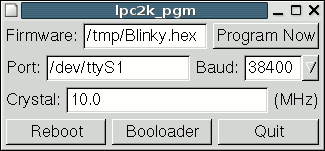
\includegraphics[width = 0.4\columnwidth]{img/lpc2k_pgm}}&%
			
		\subfigure[Terminal serie de la uart0]{
			\label{fig:lpc2k_pgm_term}
			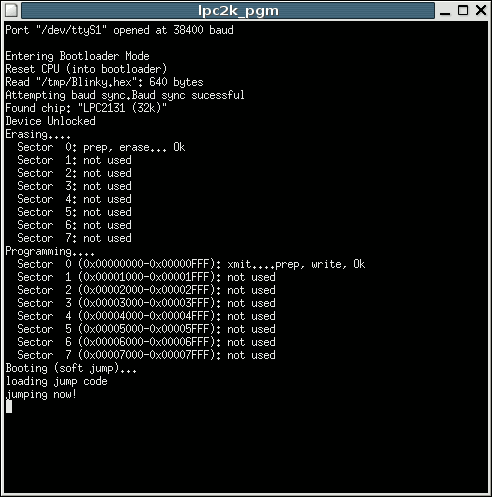
\includegraphics[width = 0.4\columnwidth]{img/lpc2k_pgm_term}}\\
	\end{tabular}
		
	\caption{Ventana de configuración y terminal serie de la uart0 del LPC2000}
	\end{center}
	\end{figure}
	
	Tras ajustar correctamente los parámetros del cargador, al ejecutar la orden de programar, nos aparecerá una ventana de terminal por la que se vuelca la salida del puerto serie UART0 del LPC2000.
	
	Como se puede observa en la imagen~\ref{fig:lpc2k_pgm}, la extensión del fichero cargado es ``.hex''. Esto se debe a que el contenido del fichero imagen cargado en la ROM debe estar en formato ihex (\emph{Intel Hexadecimal})~\cite{ihex}.

	Todos nuestro programas deberán ser traducidos del formato ELF (formato por defecto producido por el linker en el entorno Linux) a ihex. Para ello disponemos de la herramiento \texttt{objcopy}.

	%Una vez compilado nuestro programa, el resultado de la compilación  
	%será un fichero ELF (\emph{Executable and Linkable Format}) que contendrá el código del programa que mediante la herramienta \texttt{objcopy} tiene que ser convertido a ihex.
	
	\subsubsection{Conexión serie con FTDI}

	Por la parte hardware es necesario disponer de un cable USB a mini USB. Para poder acceder al UART serie que incorpora el sistema LPC2000, la conexión serie se proporciona a traves de USB por medio de un driver FTDI~\cite{FTDI}. Por ello es necesario disponer de un driver USB con soporte para FTDI en el host (PC) que se está utilizando como plataforma de desarrollo. Este driver permitirá usar la conexión serie. En el caso de GNU/Linux se ha utilizado el módulo usbserial (con soporte FTDI) que trás cargarse proporciona el dispositivo /dev/ttyUSB0, a traves del que se puede comunicar a traves del puerto serie.
	
	
	\subsection{Configuración de \partikle{}}
			
	Una vez instalado correctamente el compilador cruzado, podemos pasar a obtener y configurar \partikle{} \cite{partikleos}.
	
	La versión más actualizada de \partikle{} está disponible en el repositorio del grupo de investigación (\hrefx{https://www.gii.upv.es/svn/rtos/trunk/partikle}). Los fuentes de \partikle{} pueden residir en cualquier directorio. En nuestro caso, supondremos \texttt{/usr/\-src/\-partikle}.
	
	\begin{verbatim}
	$ cd /usr/src/
	$ svn co https://www.gii.upv.es/svn/rtos/trunk/partikle
	$ cd /usr/src/partikle
	$ make menuconfig
	\end{verbatim}

	Los aspectos a tener en cuenta durante la configuración son la arquitectura y la memoria dinámica disponible en el sistema:

	\begin{verbatim}
	Architecture 
	    >> LPC (arm7) Stand Alone system
	Core Options 
	    >> Kernel Dynamic Memory: 18432 bytes (18 Kbytes)
	    >> User Dynamic Memory: 10240  bytes (10 Kbytes)
	    >> Thread stack size: 512  bytes (0.5 Kbytes)
	\end{verbatim}

	Por lo tanto, se tiene que ajustar el valor THREAD\_STACKSZ, durante la configuración de \partikle{} para adaptarlos a los requisitos de la aplicación, en este caso la memoria RAM del LPC2000 es de $32$ Kbytes por lo que $512$ bytes de pila per thread puede ser un buen valor por defecto (ver figura \ref{fig:lpc-confscr}).
	
	\begin{figure}[htbp]
	\begin{center}
	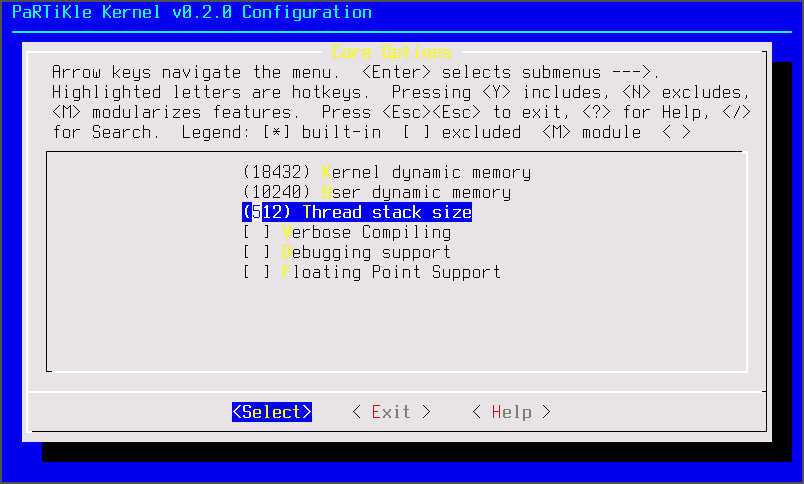
\includegraphics[width = 1\columnwidth]{img/lpc-confscr}
	\end{center}
	
	\caption{Configuración de PaRTiKle bajo el LPC2136}
	\label{fig:lpc-confscr}
	\end{figure}

	Tras realizar las anteriores selecciones podemos guardar los cambios (en el fichero .config) y salir.

	El resultado tras salir será:

	\begin{verbatim}
	>> Building the configuration utility:...

	>> End of PaRTiKle kernel configuration <<
	>> Execute 'make' to build the kernel <<
	\end{verbatim}

	Tras esto, basta con ejecutar la orden \texttt{make} para compilar \partikle{}.

	\begin{verbatim}
	$ make
	>> Detected PaRTiKle path: /usr/src/partikle
	>> Building PaRTiKle utils: done                 
	>> Building PaRTiKle kernel [lpc]: done                                    
	>> Building PaRTiKle user libraries: done                  
	
	>> Include these in your profile environment:
	   PRTK=/usr/src/partikle export PRTK
	   PATH=$PATH:$PRTK/user/bin export PATH
	\end{verbatim}
	
	\subsubsection{Introducción a \partikle{}}
	
	La interfaz básica que ofrece es la de POSIX threads PSE52 (subconjunto de servicios POSIX para sistemas mínimos).  Una característica muy interesante de \partikle{} es su modularidad, esto es, \partikle{} implementa y ofrece la interfaz POSIX-threads basándose en una interfaz con el hardware genérica. Con lo que es extremadamente sencillo ``portar'' \partikle{} a distintas arquitecturas.
	
	Buena muestra de esto es el porting de PaRTiKle a la arquitectura ARM7 para sistemas LPC que se describe en este documento. Los aspectos más destacados que facilitan las tareas de porting a nuevas arquitecturas son:
	
	\begin{enumerate}
	\item Conjunto reducido de requisitos hardware: 
		
	\begin{itemize*}
	\item initcode: código de inicialización.
	\item interrupts: manejo de interrupciones.
	\item timers: programación de timers/clocks.
	\item print: rutinas para enviar carácteres a un dispositivo de salida (vga, serie, ...)
	\end{itemize*}

	\item Proceso de configuración y compilación sencillo.

	\item Estructura del código fuente: 
	
	En el momento de programar una nueva funcionalidad para el sistema, se debe determinar si esta es común a todo el sistema (por ejemplo, planificador, gestión timers, señales, sistema de ficheros, \ldots) en dicho caso el nuevo códigos será código portable y residirá en el directorio \texttt{core/kernel/port}.
	
	Si por lo contrario se trata de código específico para una arquitectura este ocupa un directorio propio: \texttt{core/kernel/\$arch} por cada arquitectura \emph{\$arch}.
	\end{enumerate}
	
	\subsubsection{Características de \partikle{} para LPC}

	Todas las cuestiones asociadas al LPC2000 has sido ya mencionadas anteriormente.

	%Las cosas específicas de LPC que se han dicho arriba, por ej:

	Es importante remarcar que en la implementación se ha intentado minimizar la cantidad de código ensamblador escrito, para ello se ha utilizado únicamente en los detalles de inicialización donde era imprescindible utilizar ensamblador.  Como resultado utilizando la herramienta SLOCcount (SLOC: \emph{Source Lines Of Code}) se puede comprobar que:

	\begin{verbatim}
	% cd /usr/src/partikle/core/kernel/lpc/
	% sloccount .
	SLOC    Directory       SLOC-by-Language (Sorted)
	1511    lpc             ansic=1410,asm=101
	
	Totals grouped by language (dominant language first):
	ansic:         1410 (93.32%)
	asm:            101 (6.68%)
	\end{verbatim}
	
	Básicamente, el código ensamblador escrito se encarga de preparar un contexto para poder llamar a la primera función C, para llevar a cabo el resto de la inicialización por medio de código escrito en C, por medio de lecturas/escrituras sobre registros.
		
	\subsubsection{Programación de aplicaciones \partikle{}}
	
	Una vez terminado el anterior paso, ya podemos utilizar \partikle{} para desarrollar aplicaciones con el LPC2000.
	A modo de ejemplo podemos compilar y ejecutar los ejemplos que se distribuyen con PaRTiKle (se encuentran en \texttt{user/\-examples/\-c\_examples}):.
	
	\begin{verbatim}
	$ cd /usr/src/partikle
	$ cd user/examples/c_examples
	$ make
	\end{verbatim}
	
	Tras esto se compilarán los programas ``.c'' contenidos en el directorio actual, el resultado será un fichero ``.prtk'' por cada ``.c'', los ficheros ``.prtk'' contienen el ejecutable del programa en formato ELF, para poder ser cargados en el LPC2000 utilizando el lpc2k\_pgm han de ser convertidos a Intel Hex, lo que se realiza mediante la orden \texttt{make}:

	\begin{verbatim}
	$ make hello_world.hex
	\end{verbatim}
	
	para luego utilizar el cargador flash, para transmitirlo al LPC2000 y ejecutarlo,
	ver la siguiente captura de pantalla (figura \ref{fig:lpc-bootscr}) del proceso de carga y ejecución:

	\begin{verbatim}
	$ lpc2k_pgm
	\end{verbatim}
	
	\begin{figure}[htbp]
	\begin{center}
	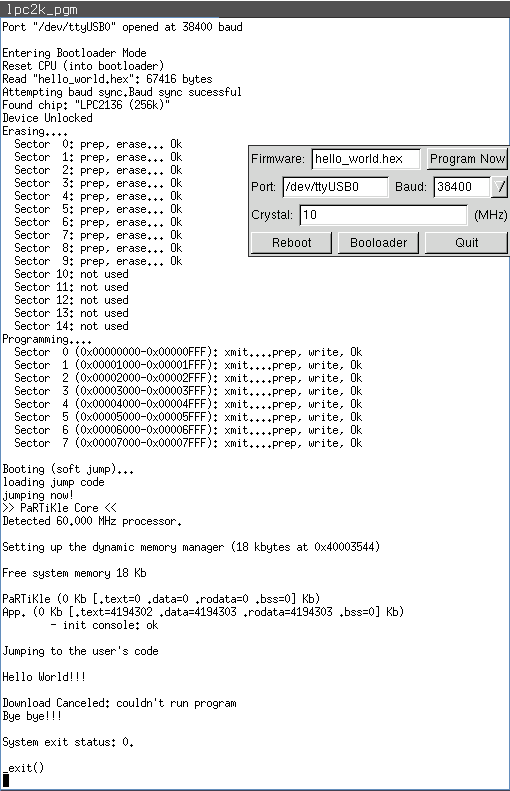
\includegraphics[width = 1.0\columnwidth]{img/lpc-bootscr}
	\end{center}
	
	\caption{Arranque de PaRTiKle bajo el LPC2136}
	\label{fig:lpc-bootscr}
	\end{figure}

\newpage

% la bibliografía empleada
\begin{thebibliography}{1}
\selectlanguage{english}

% links de partikle
\bibitem[1]{partikleos}
	S. Peiro, M. Masmano, I. Ripoll, and A. Crespo,
	\newblock { \em{PaRTiKle OS, a replacement of the RTLinux core}}.
	\newblock Real-Time Systems Group, Universidad Politécnica de Valencia.
	\hrefx{http://www.e-rtl.org/partikle/node/5},
	\hrefx{http://www.e-rtl.org/partikle}.
	
\bibitem[2]{partikle-um}
	M. Masmano, I. Ripoll, A. Crespo,
	\newblock { \em{PaRTiKle OS User Manual}}.
	\newblock Real-Time Systems Group, Universidad Politécnica de Valencia.
	\hrefx{http://www.e-rtl.org/partikle/node/5}.
	
\bibitem[3]{xtratum}
	M. Masmano; I. Ripoll, A. Crespo, 
	\newblock {\em {An overview of the XtratuM nanokernel}}, 
	\newblock  Workshop on Operating Systems Platforms for Embedded Real-Time applications, (2005),
	\hrefx{http://www.xtratum.org/biblio}.

% links de LPC
\bibitem[4]{lpc213x-um}
	NXP,
	\newblock { \em {LPC2131/2/4/6/8 User manual}}.
	\newblock NXP, founded by Philips,
	\newblock \hrefx{http://www.standardics.nxp.com/support/documents/microcontrollers/?search=LPC2\&type=user}.

\bibitem[5]{tigtarm7}
	Trevor Martin,
	\newblock { \em {The Insider's guide to the ARM7-based microcontrollers}}.
	\newblock Hitex development tools,
	\hrefx{http://hitex.co.uk/arm}.

\bibitem[6]{arm7tdmi-s}
	Advanced RISC Machines,
	\newblock { \em{ARM7TDMI-S (rev r4p3) Technical Reference manual}}.
	\newblock ARM Limited.
	\hrefx{http://www.arm.com/documentation/ARMProcessor\_Cores}.

\bibitem[7]{armarm}
	David Seal,
	\newblock { \em{The ARM Architecture Reference Manual}}.
	\newblock 2nd Edition, Addison-Wesley Longman Publishing Co.
	\hrefx{http://www.arm.com/documentation/books.html}.

\bibitem[8]{lpc2000ans}
	NXP,
	\newblock { \em{LPC2000 Application Notes, Boot sequence, Interrupts, Spurious Interrupts}}.
	\newblock NXP, founded by Philips.
	\hrefx{http://www.standardics.nxp.com/support/documents/microcontrollers/?search=LPC2}.

\bibitem[9]{lpc2k_pgm}
	Paul Stoffregen,
	\newblock { \em{LPC2K\_PGM Linux Bootloader Utility (Philips LPC 2000 ARM7 Chips)}}.
	\hrefx{http://www.pjrc.com/arm/lpc2k\_pgm}.

% misc links
\bibitem[10]{mikro}
	\newblock { \em{The Mikrocontroller project}},
	\hrefx{http://www.mikrocontroller.net/articles/LPC2000}.
	
\bibitem[12]{lpc-examples}
	Martin Thomas,
	\newblock { \em{Philips LPC213x/214x examples ported for the GNU-Toolchain}},
	\hrefx{http://www.siwawi.arubi.uni-kl.de/avr\_projects/arm\_projects/lpc2k\_bundle\_port/}.

\bibitem[13]{ihex}
	Intel Corporation,
	\newblock { \em{Intel Hexadecimal Object File Format Specification}},
	\newblock  Intel 1988, 
	\hrefx{http://www.pjrc.com/tech/8051/pm2\_docs/intel-hex.html}.

	
\bibitem[14]{FTDI}
	Craig Peacock,
	\newblock {\em USB with the simplicity of RS-232}
	\hrefx{http://www.beyondlogic.org/usb/ftdi.htm}.

\bibitem[15]{UART}
	Craig Peacock,
	\newblock {\em Interfacing the Serial / RS-232 Port}
	\hrefx{http://www.beyondlogic.org/serial/serial.htm}

\bibitem[16]{ATCPS}
	Development systems Division, Compiler Tools Group
	\newblock {\em Procedure Call Standard for the ARM Architecture}.
	\newblock  ARM Limited, 2003.
	\hrefx{http://infocenter.arm.com/help/topic/com.arm.doc.ihi0042a/IHI0042A\_aapcs.pdf}
	
\bibitem[17]{lamport}
            Leslie Lamport.
            \newblock {\em {\LaTeX:} {A} Document Preparation System.
            (User's Guide and Reference Manual)}.
            \newblock Addison-Wesley, Reading, Massachusetts, second edition, 1986.
\end{thebibliography}


\end{document}
